
\section{题集}

\begin{exercise}
\label{exercise:2016-06-24-1}
  如图,在三角形$ABC$中,$AO$是$BC$边上的高,$D$是$AO$的中点,点$E$是其内切圆$\odot I$与$BC$边的切点,连接$ED$并延长与内切圆相交于另一点$F$,过点$C$并与$BC$垂直的直线与$BI$的延长线相交于$G$,求证:(1) $EF \perp FG$,(2)$EF$平分角$BFC$。
\end{exercise}
\begin{figure}[htbp]
  \centering
\includegraphics{content/plane-geometry/pic/2016-06-24-1.pdf}
\caption{}
\label{fig:2016-06-24-1}
\end{figure}

\begin{exercise}
  如图\ref{fig:2017-02-09-01-01},分别以三角形$ABC$的边$AB$和$AC$向形外作正方形,两个正方形的中心分别记为$O_{1}$和$O_{2}$,$X$是$BC$边中点,其余各点的意义如图所示,求证:
  \begin{enumerate}
  \item 三角形$O_{1}XO_{2}$是等腰直角三角形.
  \item $ST \parallel PQ$.
  \end{enumerate}
\end{exercise}

\begin{figure}[htbp]
  \centering
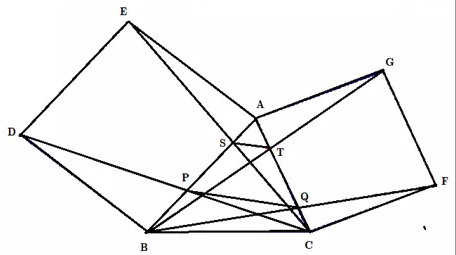
\includegraphics[scale=0.6]{content/plane-geometry/pic/2017-02-09-01-01.png}
\caption{}
\label{fig:2017-02-09-01-01}
\end{figure}
  
\begin{proof}[证明]
  易见$\triangle ACE \cong \triangle AGB$,而$O_{1}X \parallel EC$并且$|O_{1}X|=\frac{1}{2}|EC|$,同样$O_2X \parallel BG$并且$|O_2X|=\frac{1}{2}|BG|$,但是$EC=BG$,并且$EC \perp BG$,所以$O_1X=O_2X$并且$O_1X \perp O_2X$,所以$\triangle O_{1}XO_{2}$是等腰直角三角形.

  第二问的最简单证法是设$DE$延长线与$CA$延长线交于$U$,$FG$延长线与$BA$延长线交于$V$,则有 $\triangle AEU \sim \triangle AGV$,于是
  \begin{equation*}
    \frac{AS}{SP}=\frac{UE}{ED}=\frac{UE}{EA}=\frac{VG}{GA}=\frac{VG}{GF}=\frac{AT}{TQ}
  \end{equation*}
  所以$ST \parallel PQ$.

\begin{figure}[htbp]
  \centering
\includegraphics{content/plane-geometry/pic/2017-02-09-01-02.pdf}
\caption{}
\label{fig:2017-02-09-01-02}
\end{figure}

  如果注意到图中包含着两个同样的基本图形,则可以有如下的证明,先提一个引理:如图\ref{fig:2017-02-09-01-02},设点$P$为正方形$ABCD$的边$AB$外侧一点,$PC$与$PD$分别与边$AB$相交于$S$和$T$,记$\angle PAB=\alpha, \angle PBA=\beta$,则有
  \begin{equation*}
    AT : TS : SB = \cos{\alpha}\sin{\beta} : \sin{\alpha}\sin{\beta} : \sin{\alpha}\cos{\beta}
  \end{equation*}
  利用此引理知,$AT:TS$仅与角$\alpha$有关,因此在原题中立刻便有$\frac{AS}{SP}=\frac{AT}{TQ}$,因此两线平行,而这个引理的证明也很简单,记点$P$在边$AB$上的投影为$R$,并假定正方形边长为1,并记$PB=a, PA=b$,根据正弦定理可得 
  \begin{equation*}
    \frac{a}{\sin{\alpha}}=\frac{1}{\sin{\alpha+\beta}}=\frac{b}{\sin{\beta}}
  \end{equation*}
  于是
  \begin{equation*}
    a=\frac{\sin{\alpha}}{\sin{\alpha+\beta}}, b=\frac{\sin{\beta}}{\sin{\alpha+\beta}}
  \end{equation*}
  根据几何关系有
  \begin{equation*}
    AR=b\cos{\alpha}=\frac{\cos{\alpha}\sin{\beta}}{\sin{\alpha+\beta}}, PR=b\sin{\alpha}=\frac{\sin{\beta}}{\sin{\alpha+\beta}}
  \end{equation*}
  而由$\frac{TR}{AT}=\frac{PR}{AD}$得
  \begin{equation*}
    AT=\frac{AT}{AT+TR}AR=\frac{1}{1+\frac{TR}{AT}}AR
    = \frac{1}{1+\frac{\sin{\alpha}\sin{\beta}}{\sin{\alpha+\beta}}} \cdot \frac{\cos{\alpha}\sin{\beta}}{\sin{\alpha+\beta}}
    = \frac{\cos{\alpha}\sin{\beta}}{\sin{\alpha}\sin{beta}+\sin{\alpha+\beta}}
  \end{equation*}
  根据对称性,互换$\alpha$和$\beta$可得
  \begin{equation*}
    BS = \frac{\sin{\alpha}\cos{\beta}}{\sin{\alpha}\sin{\beta}+\sin{\alpha+\beta}}
  \end{equation*}
  于是
  \begin{equation*}
    TS = \frac{\sin{\alpha}\sin{\beta}}{\sin{\alpha}\sin{\beta}+\sin{\alpha+\beta}}
  \end{equation*}
  于是引理得证。
\end{proof}

%%% Local Variables:
%%% mode: latex
%%% TeX-master: "../../book"
%%% End:
